\chapter{Setup}
Since the VGG-Face only accepts images, the videos must be converted by extracting frames from the videos and using those frames as inputs to the neural network. To obtain better results, a multi-modality approach is also considered. The model must be tweak to accept non-image inputs using middle fuse strategies to combine both inputs.

%%%%%%%%%%%%%%%%%%%
% SECTION FAKE VS REAL
%%%%%%%%%%%%%%%%%%%
\section{Fake vs Real}

\subsection{Pre-processing}

The SASE-FE was pre-processed to extract each frame as an image. Because the SASE-FE videos start with a neutral face expression and then the participant makes the facial expression corresponding to the emotion, there are some frames which are of no use. The pre-processing considers this and only keep the frames from half of the video duration until the 80\% of the video duration. This ensures that the frames obtained shows the intended emotion.

A second transformation to the SASE-FE dataset was conducted using a process called frontalization, introduced by Hassner et al \cite{HassnerEffectiveImages}. This method rotates and scales the face of the participant thus reducing the variability of the position of the faces by changing unconstrained viewpoints to constrained, forward facing faces. Frontalization can help reduce variability but it also has some drawbacks specially when the face has some partial occlusion. Hassner also introduces soft symmetry that allows occluded parts of the face to be estimated when both parts of the face are different. Blending methods are employed obtain an image that is symmetrical on both sides.

% FIGURE: symmetry
\begin{figure}[H]
    \centering
	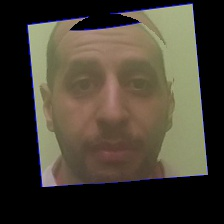
\includegraphics[width=0.4\textwidth]{nosymmetry.jpg}
	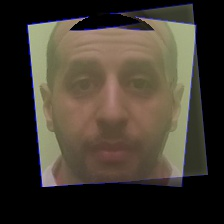
\includegraphics[width=0.4\textwidth]{softsymmetry.jpg}    
    \caption{Right image shows an image with No Symmetry frontalization. Left image corresponds to a Soft Symmetry frontalization process.}
    \label{image:symmetry}
\end{figure}

To perform frontalization, Hassner method \cite{HassnerEffectiveImages} obtains face landmarks which consist of 68 fiducial points. These features correspond to points in the mouth, nose, eyes, etc. These landmarks are then used as a second input to the VGG-Face model. A middle fusion strategy is required in the first fully connected layers since the VGG-Face only accepts images as input.

% FIGURE: geometry
\begin{figure}[H]
    \centering
	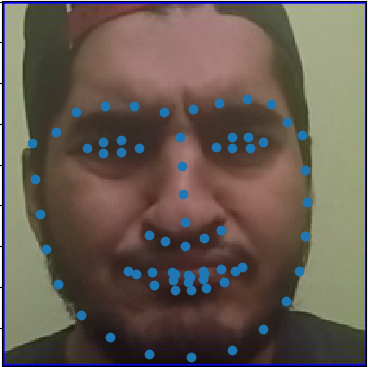
\includegraphics{geometry.png}
    \caption{68 fiducial points overlay on the detected face.}
    \label{image:geometry}
\end{figure}

%%%%%%%%%%%%%%%%%%%
% SECTION BLOCKED VS REAL
%%%%%%%%%%%%%%%%%%%
\section{Blocked vs Real}

\subsection{Pre-processing}
